\section{Taxonomy and Overview}
\label{sec:taxonomy}

To systematically classify the rapidly expanding body of literature on scientific multimodal time series foundation models and reasoning LLMs, we construct a four-dimensional taxonomy framework, as illustrated in Fig.~\ref{fig:taxonomy_tree}. Unlike general-purpose temporal surveys that divide models simply by task (e.g., forecasting vs. imputation), our categorization captures the unique physical, mathematical, and algorithmic requirements of scientific domain applications.

\begin{figure*}[t]
\centering
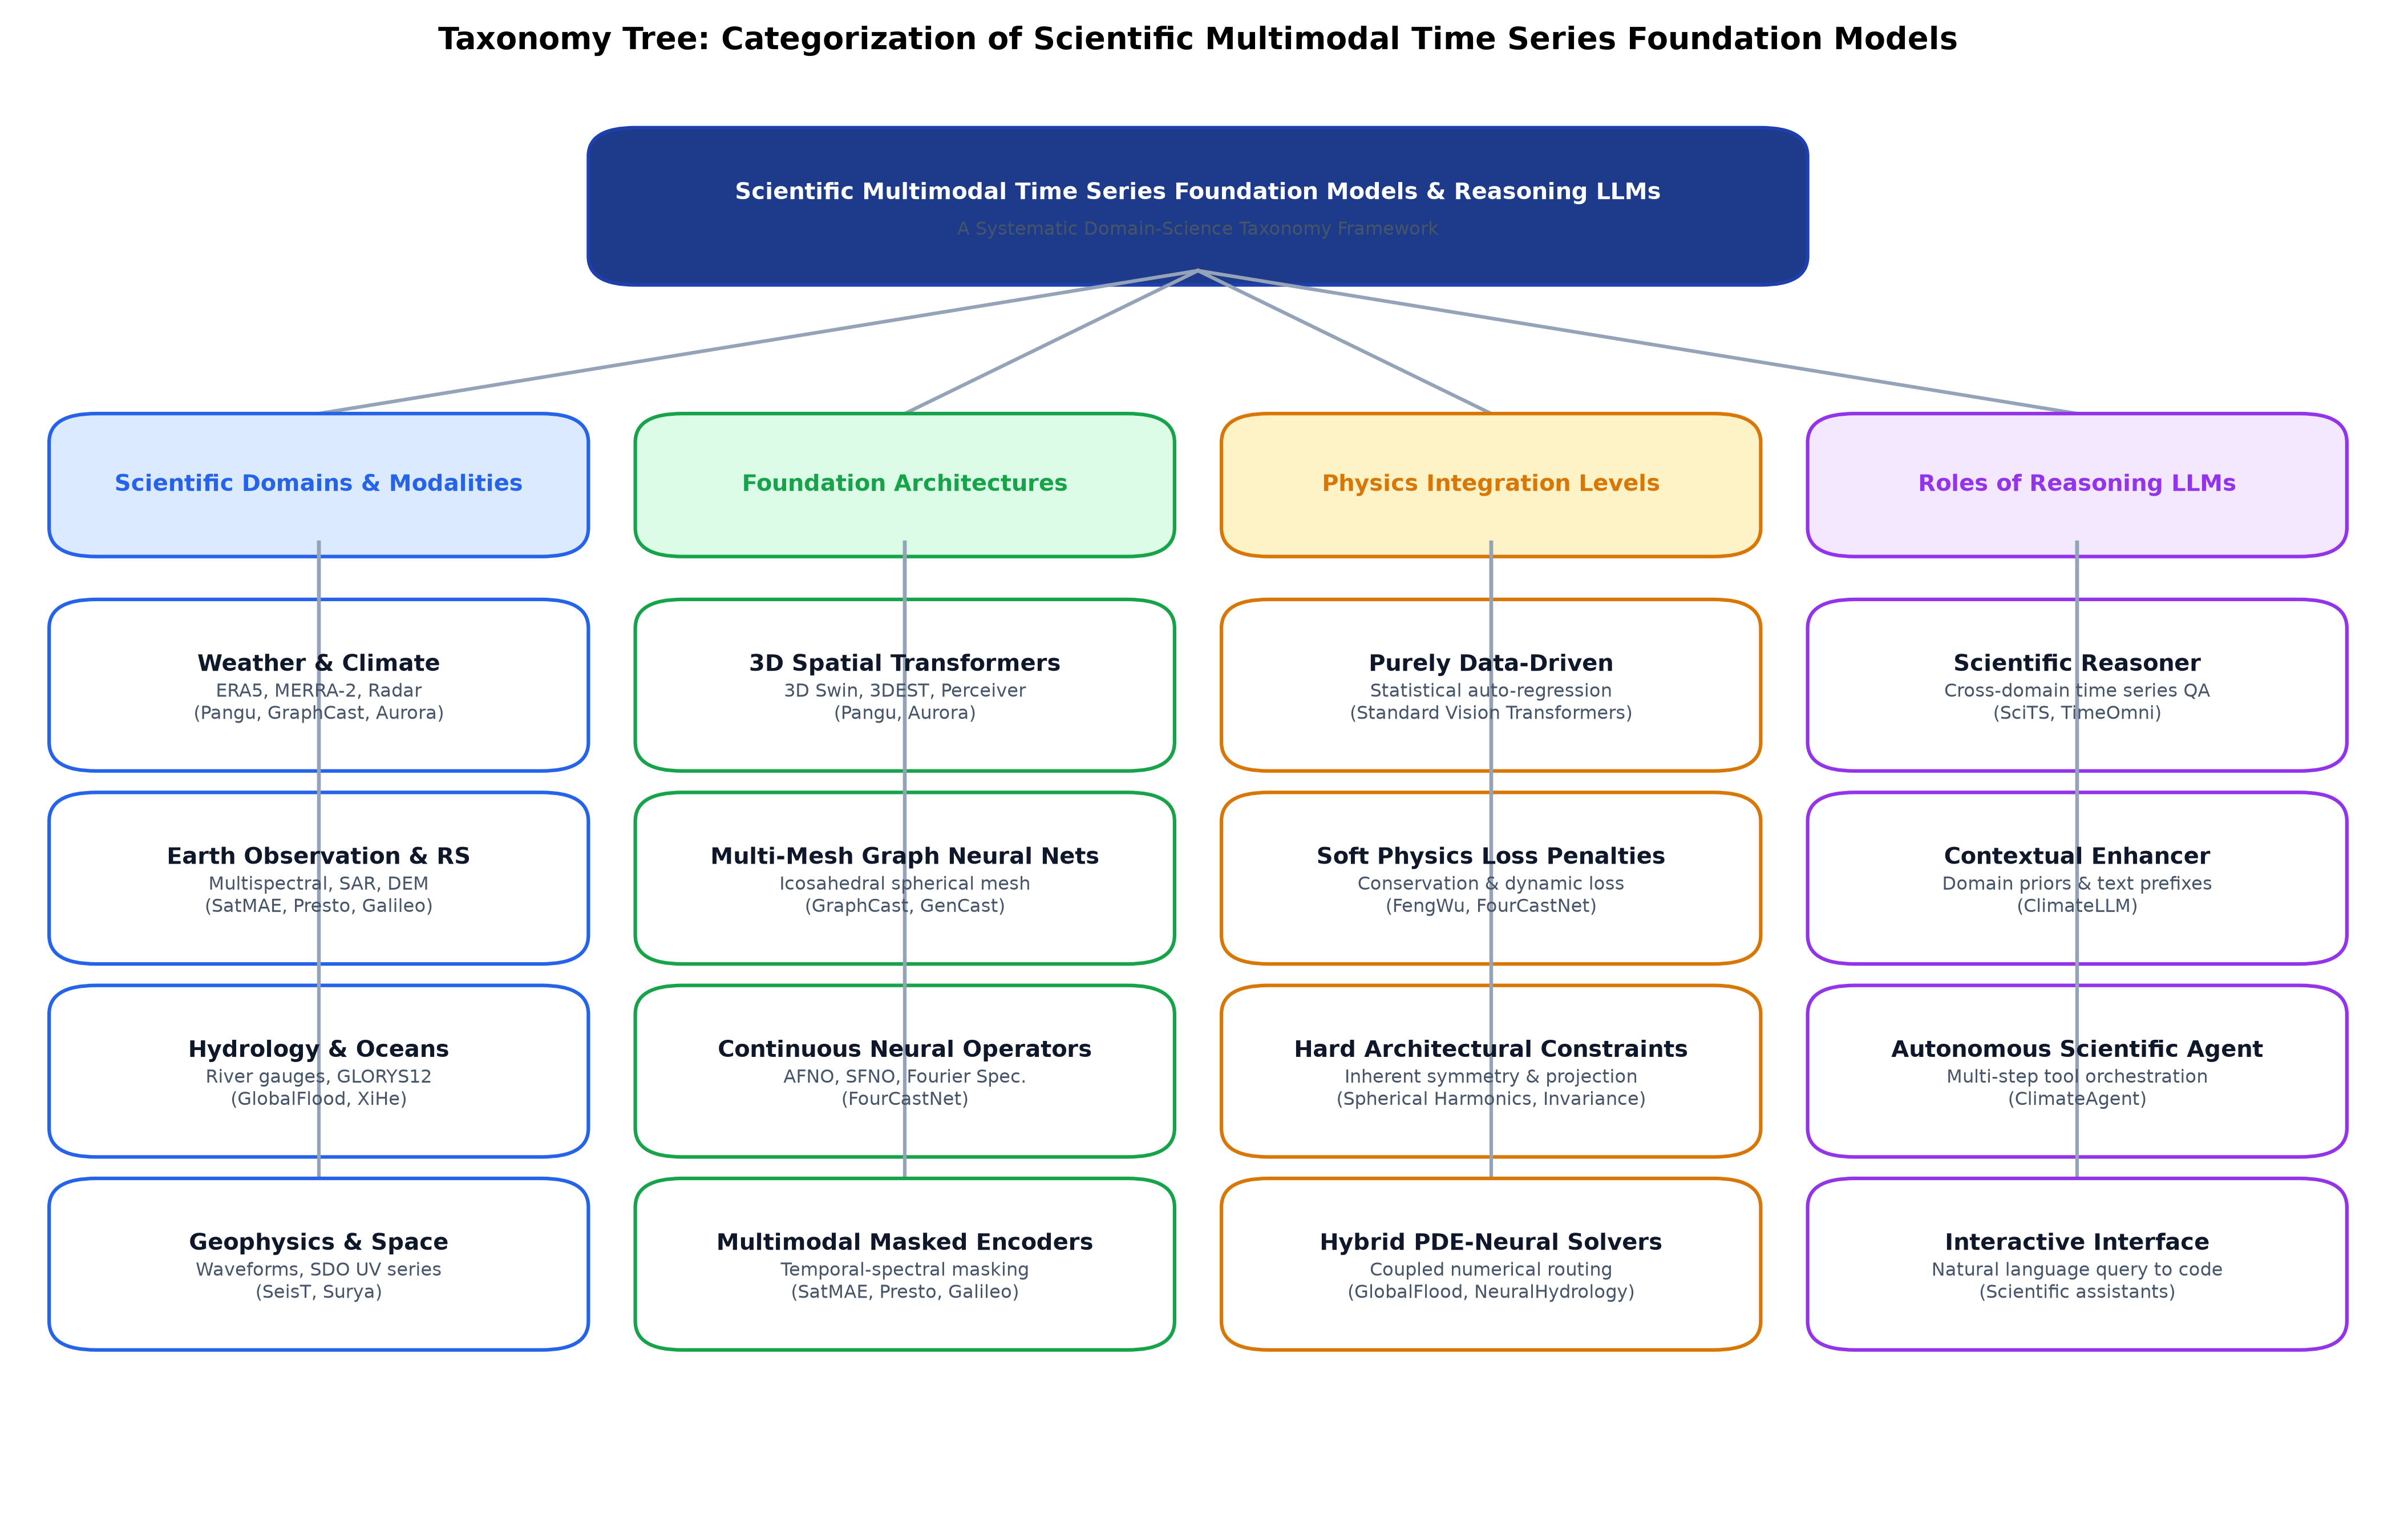
\includegraphics[width=\textwidth]{figures/taxonomy_tree.png}
\caption{Comprehensive taxonomy framework for scientific multimodal time series foundation models and reasoning LLMs, structured across four orthogonal dimensions: Scientific Domains \& Modalities, Foundation Architectures, Physics Integration Levels, and Roles of Reasoning LLMs.}
\label{fig:taxonomy_tree}
\end{figure*}

\subsection{Dimension 1: Scientific Domains and Modalities}
Scientific time series foundation models specialize across distinct physical environments:
\begin{itemize}
    \item \textbf{Weather and Climate}: Characterized by 3D spherical atmospheric reanalysis fields (ERA5, MERRA-2, IFS HRES), satellite radiometer scans, and ground radar nowcasting sequences~\cite{bi2023pangu,lam2023graphcast,pathak2022fourcastnet,bodnar2024aurora}.
    \item \textbf{Earth Observation and Remote Sensing}: Composed of irregular multi-spectral satellite revisit series (Sentinel-1 SAR, Sentinel-2 Optical, Landsat-8), high-resolution elevation maps, and surface reflectance temporal trajectories~\cite{cong2022satmae,tseng2023presto,tseng2025galileo,jakubik2023prithvi,brown2025alphaearth}.
    \item \textbf{Hydrology and Water Resources}: Integrating multi-basin river streamflow gauges, topological river drainage networks, and gridded surface precipitation/evapotranspiration dynamics~\cite{nearing2024globalflood}.
    \item \textbf{Oceanography and Marine Systems}: Involving global eddy-resolving reanalysis fields (e.g., GLORYS12V1), sea surface height anomalies, temperature/salinity profiles, and acoustic sensor logs~\cite{wang2024xihe}.
    \item \textbf{Geophysics and Seismology}: Continuous 3-component seismic waveforms, phase arrival triggers, fault slip observations, and GPS tectonic deformation velocities~\cite{li2024seist,zhu2019phasenet}.
    \item \textbf{Space Weather and Heliophysics}: Continuous solar extreme ultraviolet (EUV) magnetograms, solar wind ion velocities, and geomagnetic disturbance indices~\cite{roy2025surya}.
\end{itemize}

As visualized in the Domain $\times$ Modality Research Maturity Matrix (Fig.~\ref{fig:domain_modality_heatmap}), while gridded weather reanalysis and multi-spectral satellite imagery have achieved high maturity, cross-modal integration (e.g., coupling continuous waveforms with satellite imagery or ground gauges with scientific text logs) remains an active frontier.

\begin{figure}[t]
\centering
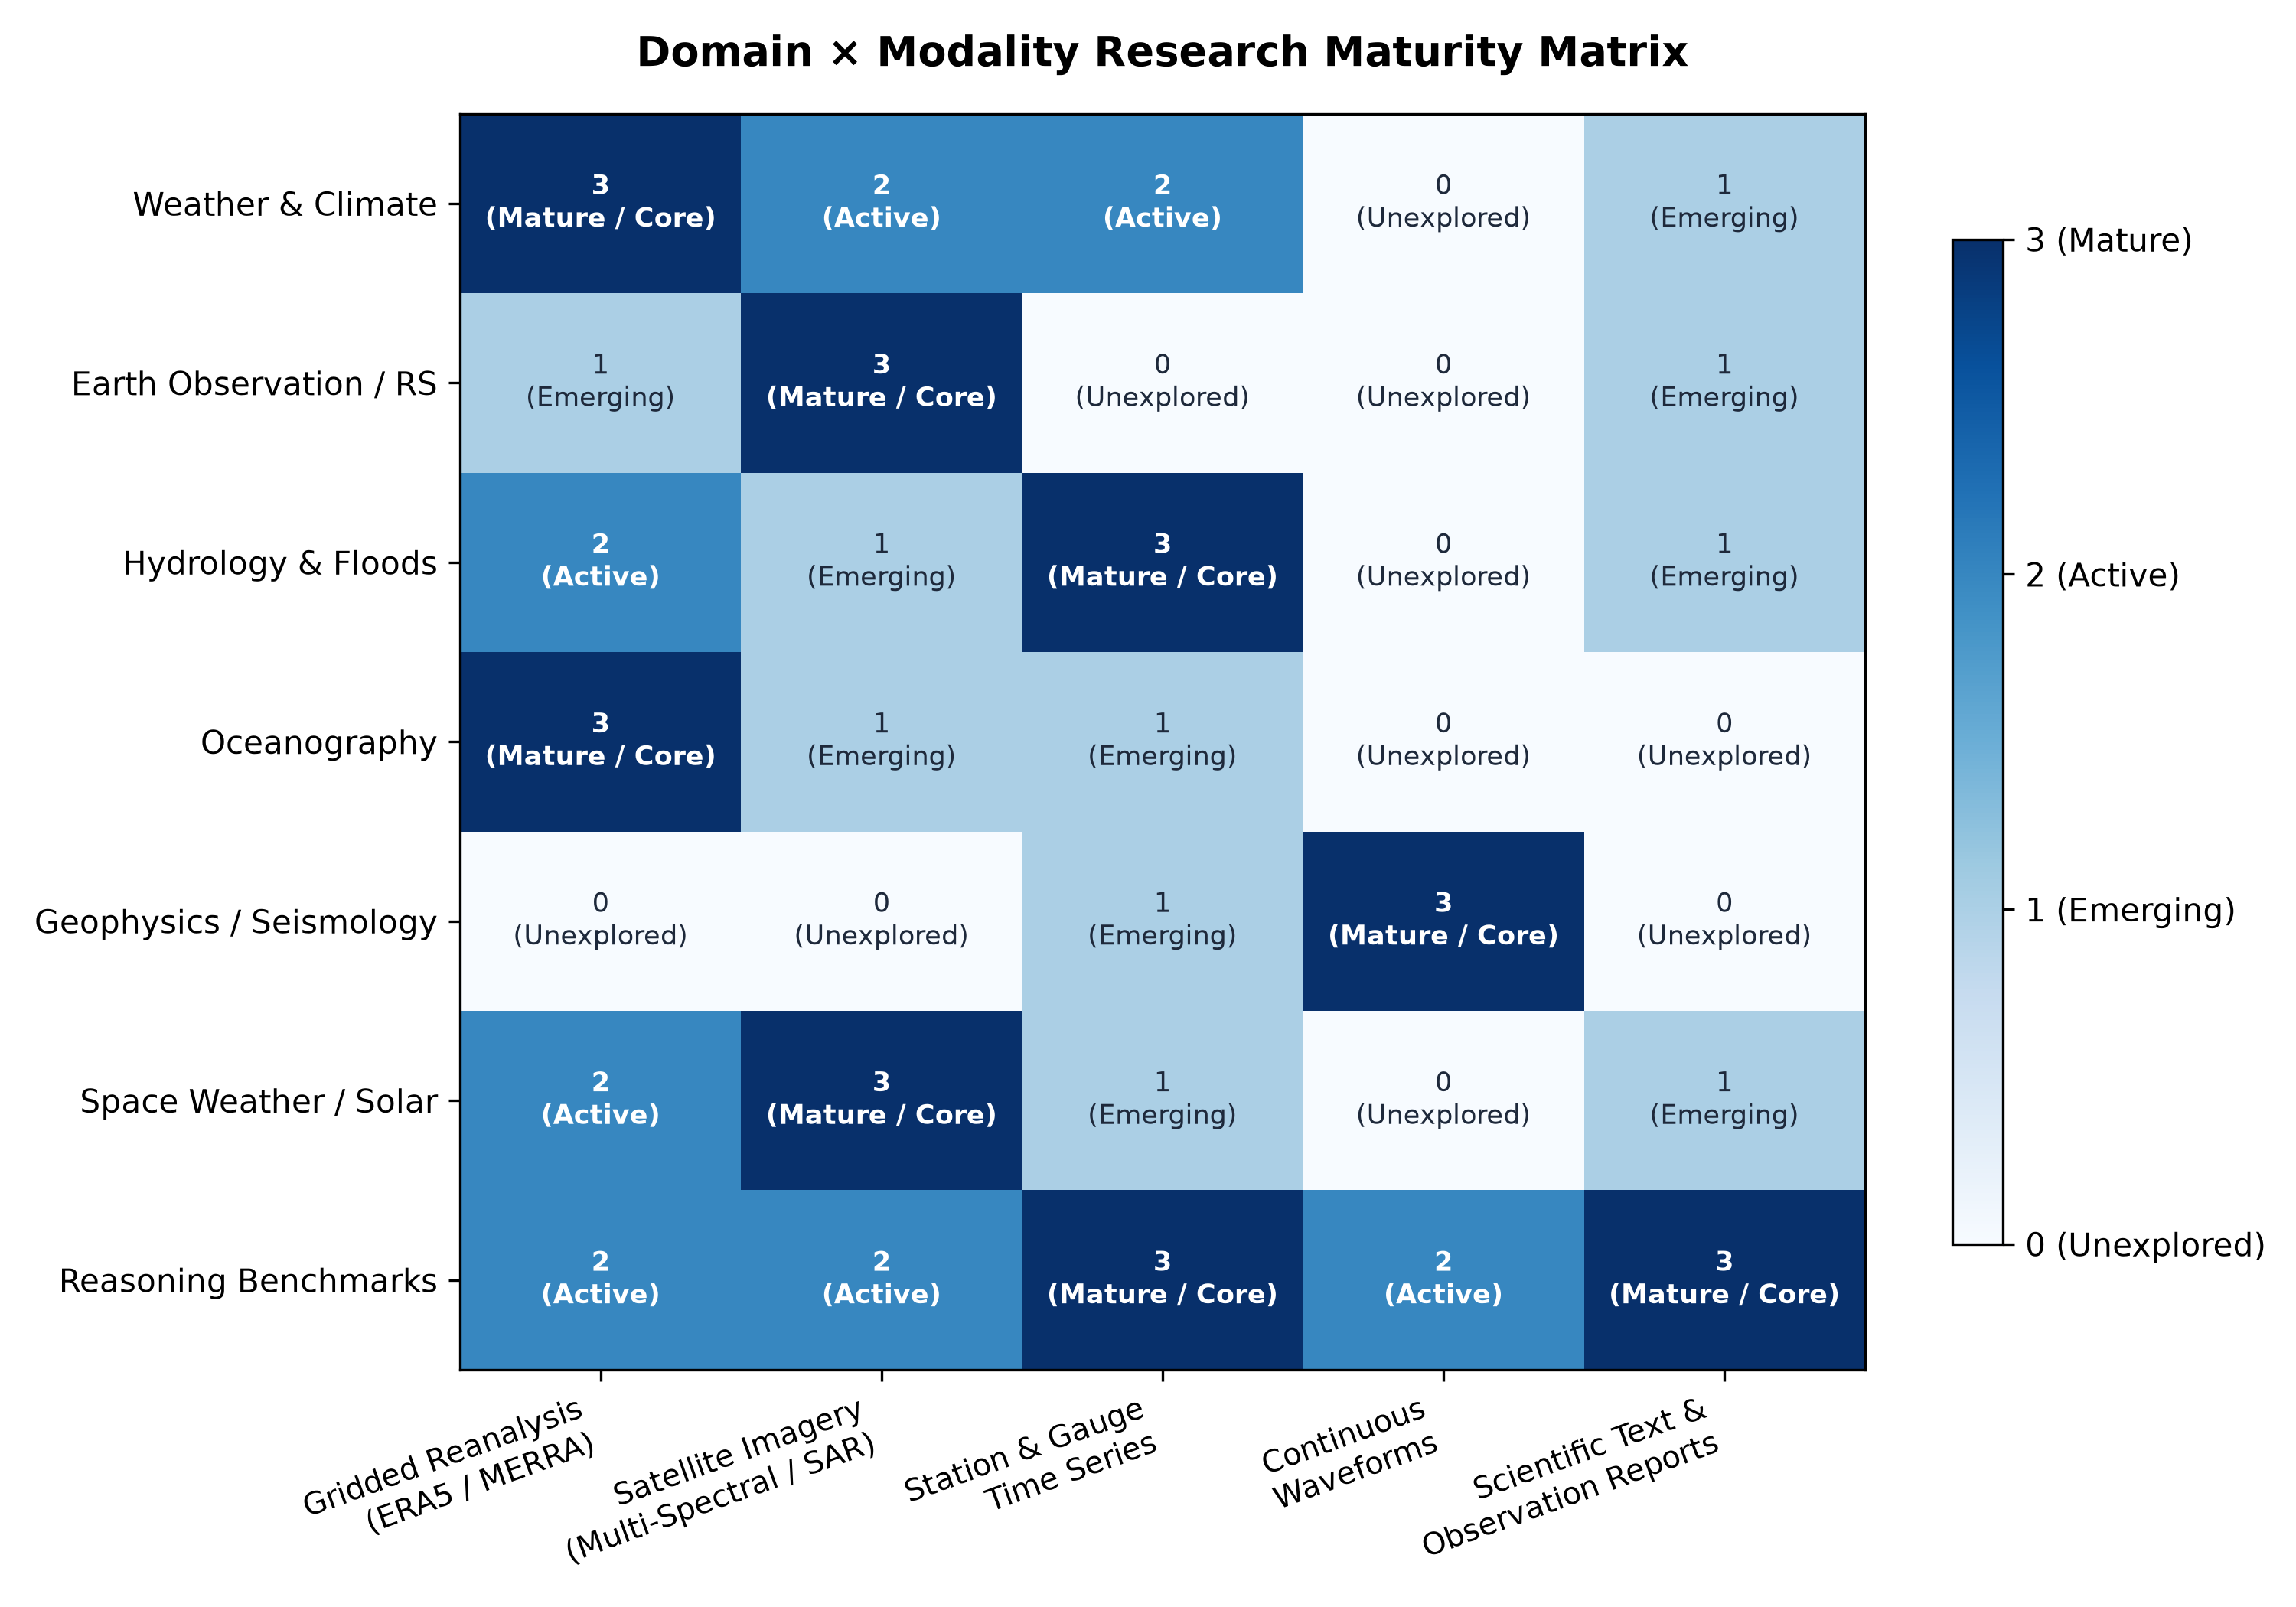
\includegraphics[width=\columnwidth]{figures/domain_modality_heatmap.png}
\caption{Domain $\times$ Modality Research Maturity Matrix, highlighting established core areas and emerging multimodal frontiers.}
\label{fig:domain_modality_heatmap}
\end{figure}

\subsection{Dimension 2: Foundation Model Architectures}
We categorize foundation backbones by their spatial-temporal inductive biases:
\begin{itemize}
    \item \textbf{3D Spatial Transformers}: Employing 3D Earth-specific patch embeddings, hierarchical Swin-like windowed attention, and vertical pressure-level encodings~\cite{bi2023pangu,bodnar2024aurora,chen2023fuxi}.
    \item \textbf{Multi-Mesh Graph Neural Networks}: Discretizing the spherical Earth via refined recursive icosahedral meshes to ensure uniform spatial resolution without polar distortions~\cite{lam2023graphcast}.
    \item \textbf{Continuous Neural Operators}: Leveraging Fourier transforms and spectral convolutions (e.g., AFNO, SFNO) to learn discretization-invariant operators on function spaces~\cite{pathak2022fourcastnet}.
    \item \textbf{Multimodal Masked Autoencoders}: Extending masked autoencoding (MAE) across spatial patches, temporal revisit cycles, and spectral channel wavelengths~\cite{cong2022satmae,tseng2023presto,tseng2025galileo,jakubik2023prithvi}.
    \item \textbf{Generative Diffusion Models}: Utilizing score-based diffusion denoising to generate calibrated, physically perturbed probabilistic weather and extreme event ensembles~\cite{price2023gencast}.
\end{itemize}

\subsection{Dimension 3: Physics Integration Levels}
The physical fidelity of deep learning models ranges along four distinct levels:
\begin{enumerate}
    \item \textbf{Purely Data-Driven}: Models optimize statistical reconstruction (e.g., mean squared error, MAE) over historical datasets without explicit differential constraints, relying solely on model capacity to reflect physical dynamics.
    \item \textbf{Soft Physics Loss Penalties}: Physical conservation principles (e.g., kinetic energy conservation, mass balance, divergence-free constraints) are formulated as penalty terms within the training loss function~\cite{chen2023fengwu,pathak2022fourcastnet}.
    \item \textbf{Hard Architectural Conservation Constraints}: Structural projections (e.g., spherical harmonics basis expansion, divergence-free projection layers) guarantee that model predictions strictly satisfy conservation laws by construction.
    \item \textbf{Hybrid PDE-Neural Ensembles}: Deep neural representations predict intermediate flux states or residual tendencies coupled directly to numerical differential equation solvers~\cite{nearing2024globalflood}.
\end{enumerate}

\subsection{Dimension 4: Functional Roles of Reasoning LLMs}
Large Language Models engage with scientific temporal data through four operational archetypes:
\begin{itemize}
    \item \textbf{Scientific Reasoner}: Understanding physical time series tokens and generating natural language explanations, causal attribution, and hypothesis evaluation across scientific domains~\cite{wu2025scits}.
    \item \textbf{Contextual Enhancer}: Supplying auxiliary domain semantics, station metadata, and climate zone priors to guide numerical prediction backbones~\cite{li2025climatellm}.
    \item \textbf{Autonomous Tool-Using Agent}: Decomposing complex scientific inquiries, retrieving real-time sensor streams, and executing scientific diagnostic libraries (e.g., CDO, xarray, SciPy) to produce verified scientific analyses~\cite{li2025climateagent}.
    \item \textbf{Interactive Natural Language Interface}: Translating unstructured scientist inquiries into executable database queries and simulation configurations.
\end{itemize}
